
%=== methology ===
% chapter-"极端质量比旋近"和”EMRI信号处理"都是属于国内外现状调研。
%\chapter{国内外相关研究综述}
%综述:针对拟研究的问题已有哪些工作和方法?
%分析:已有方法的优缺点对比,存在哪些缺陷
%归纳:方法分类,问题归纳(预示本文的工作)
%动因:阐述自己的思路,进行问题分解。
%15~20页,约1.8W字~2.4W字



%-------------------------------------------------

%论文第3~5章为主体内容。阐述自己的创新工作:理论与实验并重
%1、阐述自己最重要的创新
%2、注意几个创新点之间的关联
%3、有充分的实验对比和结果分析
%一般为50~60页,越6~7万字。

%-------------------------------------------------
\chapter{极端质量比旋近(EMRI)引力波}
%EMRI的名词解释(Extreme Mass Ratio Inspirals, EMRI)
%EMRI的波形模型:AK,AAK,AKS

本章介绍极端质量比旋近,目前对EMRI信号探测所建立的波形模型,及天琴对EMRI信号的响应和探测能力。


%\section{EMRI}
% 物理机制再补充一些,比如如何形成的损失锥,从而诱发EMRI事件
目前对银河系和河外星系研究表明,几乎每个星系中心都可能存在一个质量大约在$10^4-10^7 M_{\odot}$的黑洞。这个质量范围的黑洞也被称为大质量黑洞(Supermassive Black Hole, SMBH).在星系中心超大质量黑洞的周围,分布大量的致密天体,比如白矮星、中子星、恒星级黑洞等。当致密小天体足够靠近中心黑洞时,则其可能被中心黑洞的引力场所捕获,致使致密小天体以新的运动轨道围绕中心黑洞绕转,旋近过程中损失能量和角动量,从而辐射引力波\cite{amaro2012low,chua2017augmented},该天体源也被称为极端质量比旋近(Extreme Mass Ratio Inspirals , EMRI)。由于被捕获天体的质量大约在$1 - 100M_{\odot}$,相比之下中心黑洞质量远远超过该致密天体,由此可将该天体视为点粒子。假如假设一个$10M_{\odot}$小天体落入$10^6 M_{\odot}$黑洞视界前,旋近阶段前一年时间内将约有$10^5$次绕转圈数(cycles)。旋近轨迹类似于自由粒子做测地线运动。目前对于EMRI事件率的估计都很不准确,天琴每年观测事件数是O(1)-O(1000)\cite{Fan:2020zhy}。
%LISA给出一个参考值是每年每$Gpc^3$ 几个事件[9]。

% 绕转圈数
假设小天体绕转大质量黑洞的绕转周期为$p$,观测时长$T$为一年。则由公式$\frac{2\pi}{p}=\omega$和$\omega=2\pi f_{\rm orbit}$, 而引力波辐射频率$f_{\rm GW}$为轨道频率$f_{\rm orbit}$的2倍,则可以得到$f_{\rm GW}=\frac{2}{\rm p}$
\begin{equation}
    \label{equ:Ncycle}
    \begin{split}
    N_{cycle}&= \frac{T}{p}=\frac{1}{2}Tf_{\rm GW}  \\
    &=\frac{1}{2}\int dt f_{\rm GW}   \\
    &=\frac{1}{2}\int \frac{dt}{df_{\rm GW}} df_{\rm GW} f_{\rm GW}  \\
    &=\frac{1}{2} \frac{f_{GW}}{\dot{f_{GW}}} df_{GW}
    \end{split}
\end{equation}
取大质量黑洞为$10^6M_{\odot}$, 空间探测器灵敏度曲线大约为居中频率为$3 10^{-3} \rm Hz$ 则由\autoref{equ:Ncycle}可预估在观测时长一年内,取典型引力波频率为$10^{-4}-10^{-1}Hz$,小天体的轨道绕转圈数约为$\frac{1}{2}\times 3\times 10^7\times  10^{-3} \approx 10^4$次。


%大量观测结果暗示每个星系中心或许有一个质量大约在${10^{5} - 10^{7} M_{\odot}}$的黑洞。这个质量范围的黑洞也被称为超大质量黑洞(Supermassive Black Hole,SMBH).在超大质量星系中心黑洞的周围中,围绕了大量的致密天体,比如白矮星、恒星质量黑洞。由此中心黑洞周围常常出现多种动力学过程(包括双星的散射、双星的潮汐撕裂和巨星的剥离),这也是致密天体被中心黑洞所捕获的原因。致密天体被捕获后围绕中心黑洞绕转,旋近过程中会产生引力波\cite{AJK2017}。

\section{EMRI源天文学模型}
%描述如何构建波源的天文学分布,考虑了什么参数,考虑画出天文学分布的数学模型。
EMRI波源系统的形成受中心大质量黑洞的结构和分布情况(轻种子模型\cite{madau2001massive}、重种子模型等)以及其周围的恒星级致密小天体的分布情况(数密度尖峰、损失锥等)等因素影响,综合考虑二者结构和分布及动力学过程,EMRI事件发生率是具有很大的不确定度,基于一些观测事实和理论研究结果,目前可得到部分天文学模型来描述EMRI源的分布\cite{Fan:2020zhy,babak2017science}。

%在考虑建立EMRIs波源的天文学分布时,会有很多不确定的因素。其中主要考虑中心大质量黑洞的质量函数、小天体的质量函数等三个主要因素,则分别描述如下。
%考虑中心大质量黑洞的质量函数,取两种质量分布模型,分别如下。
这些EMRI源天文学模型可视为多个物理参数的联合概率分布,以用来衡量EMRI事件发生率,也方便后续定量评估该源辐射引力波的探测率(如天琴对EMRI的探测率)。具体来说,EMRI事件发生率按照事件形成过程中所需要的天文物理量(astrophysical ingredients)\cite{babak2017science}来分步描述。第一,考虑中心大质量黑洞质量$M$的概率分布,且$M \in [10^4, 10^7] M_{\odot}$;中心黑洞质量函数的随红移的演化及中心黑洞的自旋分布。第二,大质量黑洞落在数密度尖峰结构中的比例,这会影响EMRI的形成。第三,单个大质量黑洞的EMRI事件发生率,以及形成EMRI源之后的致密小天体的质量和偏心率分布。

基于基本观测事实和分析,考虑不同的理论模型,则上述每一步的物理量可能存在多种模型。下面进行分开陈述。
%大质量黑洞的分布
由于中心大质量黑洞分布的不确定性(如大质量黑洞种子黑洞不同分为轻种子模型和重种子模型),目前大质量黑洞质量函数可分为``Barausse12"\cite{shankar2008self,shankar2013black}和``Gair10"\cite{gair2010lisa}。中心黑洞自旋$a$也会影响EMRI事件发生率。在空间探测器灵敏频段内,不同中心黑洞质量的中心黑洞角动量和吸积盘角动量会有所不同\cite{sesana2014linking},中心黑洞更倾向于高自旋黑洞,故而定义自旋模型是``a98",即自旋的中值为0.98。为了进行比较,取另外一个自旋模型是均匀分布``aflat",和假设大质量黑洞没有自旋``a0"。
对第二步中的物理量,主要围绕中心大质量黑洞的数密度尖峰结构的模型,主要采用恒星数密度尖峰满足幂律关系$\rho(r)\propto r^{-7/4}$。但是由于星系并合,恒星数密度会被削弱。在这种情况下,不足以产生EMRI事件。故而需要考虑中心黑洞质量和其中心的弥散速度的关系,这其中采用的模型是``Gultekin09"\cite{gultekin2009m},``KormendyHo13"\cite{kormendy2013coevolution},
``GrahamScott13"\cite{graham2012black}。
第三步中,考虑每年单个大质量黑洞的EMRI事件发生率,需要考虑小天体的捕获率。这个过程中,中心质量黑洞会进行质量吸积,跟此种中心黑洞由于致密天体的坠落(plunge)数$N_p$和小天体的质量有关。故而取$N_p=0,10,100$三个模型\cite{babak2017science},以及考虑小天体质量为$m=10 M_{\odot},30M_{\odot}$\cite{woosley2002evolution}。

故而所有物理参数综合考虑之后,得到了12个天文学模型。
之后范会敏等人\cite{Fan:2020zhy}基于理想信噪比的计算评估了天琴对EMRI这类波源的探测事件率。
%按照这些天体物理量与形成过程采用的物理量,可得到12个天文学模型,
具体如表\ref{tab:astro-models}所示。在后续的工作中,我们采用了M12这个天文学模型。
\begin{table}[htbp]  
\begin{tabularx}{14.5cm}{p{1cm}p{2cm}p{1cm}p{1cm}p{2.5cm}p{1cm}p{1.5cm}|p{2cm}}  % 10cm 減去前兩個欄位寬度後,剩下的通通給   
\hline                      % 第三欄位使用,文字超出的部份會自動折行  
模型 & 质量函数  & 自旋  & 损失尖峰 & $M-\sigma$关系 & $N_p$ &致密天体质量 & EMRI事件率($yr^{-1}$)\\  
\hline  
M1 & Barausse12  & a98  & 是 & Gultekin09 & 10 &10 & 1600\\ 
M2 & Barausse12  & a98  & 是 & KormendyHo13 & 10 &10 & 1400\\
M3 & Barausse12  & a98  & 是 & GrahamScott13 & 10 &10 & 2770\\  
M4 & Barausse12  & a98  & 是 & Gultekin09 & 10 &30 & 520(620)\\ 
M5 & Gair10  & a98  & 否 & Gultekin09 & 10 &10 & 140\\
M6 & Barausse12  & a98  & 否 & Gultekin09 & 10 &10 & 2080\\ 
M7 & Barausse12  & a98  & 是 & Gultekin09 & 0 &10 & 15800\\ 
M8 & Barausse12  & a98  & 是 & Gultekin09 & 100 &10 & 180\\
M9 & Barausse12  & a98  & 是 & Gultekin09 & 10 &10 & 1530\\  
M10 & Barausse12  & a0  & 是 & Gultekin09 & 10 &10 & 1520\\ 
M11 & Gair10  & a0  & 否 & Gultekin09 & 10 &100 & 13\\
M12 & Barausse12  & a98  & 否 & Gultekin09 & 0 &10 & 20000\\ 
\hline  
\end{tabularx} 
\caption{EMRI源天文学模型中具体参数分布。第一列是中心大质量黑洞质量分布函数。第二列是中心黑洞自旋分布。第三列是数密度尖峰结构是否损失,由于星系并合,数密度尖峰结构会被破坏。第四列是星系中心黑洞质量-弥散速度关系,第五列是EMRI事件发生并合的比率。第六列是致密小天体的质量。第七列是每年EMRI事件发生率} 
\label{tab:astro-models}
\end{table} 






\section{EMRI波形}
目前主流EMRI源信号波形模型,有Kludge 波形\cite{barack2004lisa}\cite{babak2007kludge}\cite{chua2015improved}、考虑自力的波形\cite{van2018gravitational}-\cite{barack2009gravitational}、Teukolsky波形\cite{hughes2005gravitational}等等。波形越精确,计算速率越相对越慢。由于波形准确率和产生波形速率的综合考虑,应用于数据处理波形模型主要仍然是Kludge波形,包括AK波形(Analytic Kludge Waveform)\cite{barack2004lisa},NK 波形(Numerical Kludge Waveform)\cite{babak2007kludge},AAK波形(Augmented Analytic Kludge Waveform)\cite{chua2015improved}。
%总的囊括kludge波形的特点
Kludge 波形模型是在数据分析过程中强烈使用的半相对论性质的EMRI波形。


%\subsection{AK波形}
AK波形模型是由Barack和Cutler在2004年提出。
%AK波形模型是一个轨道假设为Newtonian,且低阶四极辐射的波形模型。
假设在致密小天体围着中心黑洞绕转的轨道为Newtonian 轨道,且辐射的是低阶引力波。
建立在Peters-Matthews的基础上,依据绕转轨道相关频率信息建立相应波形,主要是三种频率,一是轨道频率,一是近日点进动速率,最后是轨道平面的进动。这三者随着时间演化,从而也使得波形的分析愈加困难。

%在EMRI辐射引力波的波形模型中,一般有17个参数影响,有时候小天体相对于中心黑洞而言,相当于一个质点,所以忽略小天体的自旋,则考虑14个参数如表\ref{table2-p}所示。
采用AK波形描述一个EMRI事件的源波形,忽略致密小天体自旋的影响,需要14个源物理参数,其中包括中心大质量黑洞质量$M$,小天体质量$\mu$,中心大质量黑洞无量纲自旋角动量$S/M^2$,偏心率$e_0$,轨道面上近日点指向$\tilde{\gamma}$,轨道角动量L绕着大质量黑洞自旋S的指向角$\alpha$,黄道坐标系下源的方位角($\theta_S,\phi_S$),大质量黑洞自旋的方位坐标($\theta_K,\phi_K$),轨道角动量L与自旋S的夹角$\lambda$,波源的距离。一般会给参考时间$t$,给定初始时间$t=0$时,能得到这些物理参数的初始值。具体参数定义如表\ref{table2-p}所示。

\begin{table}[htbp]
\centering
\caption{Summary of EMRI parameters and their meaning}
\begin{tabular}{cccc} %表格7列 全部居中显示
\hline
Category     & Parameter    & Symbol   & Standard Units  \\
%\multicolumn{4}{|c|}{事件}\\  %横向合并7列单元格  两侧添加竖线
\hline
%\multirow{6}{*}{Intrinstic}&CO's mass& \nu & M\\  %纵向合并4行单元格
\multirow{6}{*}{Intrinstic}& CO'mass &$\mu$ &$M_{\odot}$\\
&SMBH's mass   & M      & $M_{\odot}$ \\
&Initial azimuthal orbital ... frequency & $\nu_0$ &Hertz \\
&Initial eccentricity&$e_0$&1 \\
&SMBH's spin &$\chi$&$M^2$ \\
&Angle between spin and... angular momentum&$\lambda$&Radian\\
\hline
\multirow{5}{*}{Extrinstic}& Ecliptic latitude &$\theta_S$ &Radian\\
&Ecliptic longitude&$\phi_S$&Radian \\
&Polar angle of spin&$\theta_K$&Radian \\
&Azimuthal angle of spin&$\phi_K$&Radian \\
&Distance to the source&$D_L$&Parse\\
\hline
\multirow{3}{*}{Phase}&Initial azimuthal orbital...phase&$\Phi_0$&Radian \\
&Initial azimuthal angle of .. orbital angular momentum&$\alpha_0$&Radian \\
&Initial direction of pericenter&$\tilde{\gamma_0}$&Radian  \\ \hline
\label{table2-p}
\end{tabular}
\end{table}



由于一开始就假定CO-SMBH系统就是一个牛顿双星模型,则小天体运行轨道模型如下:在近似椭圆轨道上,半长轴设为a,偏心率设为e, 轨道频率则为:$\nu = (2\pi M)^{-1}(M/a)^{3/2}$。在这个椭圆轨道上建立$\hat{e_1}$和$\hat{e_2}$为相互正交单位矢量。引力波振幅是${\cal{A}} \equiv{ (2 \pi \nu M)^{2/3} \mu}$
考虑探测器对振幅响应的调制,则可知,引力波的两种偏振模式在探测器响应下,振幅调制为$A_n^{+}=-[1+(\hat{L} \cdot \hat{n})^2][a_n cos(2\gamma) - b_n sin(2\gamma)],A_n^{\times} = 2(\hat{L} \cdot {\hat{n}})[b_n cos(2 \gamma) + a_n sin(2\gamma)]$
故而实际探测器响应振幅是$A^+ \equiv \Sigma_n A_n^+$和$A^{\times} \equiv \Sigma_n A_n^{\times}$。

%给出相应绕转轨道变量的演化方程
%把各项基本公式摆明。


随着人们研究深入,数值计算得到的EMRI波形在最后的最内稳定轨道(last stable orbit)并不一定是稳定且收敛的,所以2017年计算了在Kerr时空下的最内稳定轨道的位置。参考他们的工作,假设中心黑洞为Schwarzchild黑洞,则得到的波形称为AKS波形;中心黑洞是Kerr黑洞,则得到的波形称为AKK波形。
假设最后小天体会在最内稳定轨道位置之后跳入中心黑洞,其轨道半径记为$r_{lso}$
在假定初始参数一致的情况下,AKK波形比AKS波形截断更晚,即小天体坠入黑洞更晚。而且在最后坠落(plunge)阶段,体现为AKK波形离心率会比AKS波形离心率小。

%给出截断公式定义
假定中心黑洞为史瓦西黑洞,则不考虑黑洞自旋。得到的最后引力波截断频率公式如公式所示\cite{cutler1994gravitational}。
\begin{equation}
\nu_{\rm lso}= \frac{1}{2\pi \rm M } \left(  \frac{ 1-e^2}{r_{\rm LSO}/\rm M +2e }\right)^{3/2}
\end{equation}
其中``$r_{\rm LSO}$"是最内稳定轨道的半径。
在AKS截断下,$r_{\rm LSO}=6\rm M$, 只跟中心大质量黑洞质量有关。在AKK截断下,最内稳定轨道半径的计算,满足方程\ref{akk}。
%\begin{equation}
%r_{\rm LSO}/\rm M =3 \ + \ z_2 - \sqrt{\left(3-z_1)\right) left(3+z_1}
%\end{equation}
\begin{align}\label{akk}
&r_{LSO}/M=3+z_2-\sqrt{[(3-z_1)(3+z_1+2z_2)]}, \nonumber\\
&z_1=1+(1-\hat{S}^2)^{1/3}[(1+\hat{S})^{1/3}+(1-\hat{S})^{1/3}],\nonumber\\
&z_2= \sqrt{(3\hat{S}^2+z_1^2)},
\end{align}
其中``$\hat{S}$"是大质量黑洞的自旋。

%\subsection{NK}
%\subsection{NK波形}
2007年,Babak等人提出NK波形是采用Kerr测地线和用后牛顿展开(post-Newtonian(PN) expresions)演化得到的波形。在轨道时标上,致密小天体的运动是近似于测地线运动,且特征表示为椭圆轨道的近日点进动,伴随一定轨道面的Lense-Thiring进动。

这些进动效应的不同是由于运动的径向、极性和方位分量上的频率$\omega_{r,\theta,\phi}$不同。这些频率的表达式由测地线的准开普勒(quasi-Keplerian)轨道参数$\left( e,\iota,p \right)$来描述\cite{Schmidt}。

%\subsection{AAK}
%\subsection{AAK波形模型}
AAK 波形是基于AK波形和NK波形改进的波形模型。相比于NK波形采用开普勒轨道参数计算得到轨道频率,AK波形中三个轨道频率$f_{\rm orb}$是相互独立计算得到的。其中轨道频率$f_{\rm orb}$采用开普勒第三定律,与此同时其他两个进动速率$f_{\rm pesi}$和$f_{\rm LT}$是用另外的后牛顿近似得到。然而$\left( f_{\rm orb},f_{\rm peri},f_{\rm LT} \right)$并不严格等同于真实轨道频率值$\left( \omega_r,\omega_{\phi}-\omega_{r},\omega_\phi-\omega_\theta \right)$。故而相对于NK波形来说,AK波形会在相位上很快产生差异,甚至在更早期的旋近阶段。

Alvin等人提出AAK波形也是采用三种轨道频率近似于真实轨道频率组合。通过将映射中心黑洞质量$M$,黑洞自旋参数$a$和半通径(semi-latus rectum)$p$到一些非物理参数$\left( \tilde{M},\tilde{a},\tilde{p} \right)$。他们直接的关系映射可以表示如式所示。
\begin{equation}
(f_{\rm orb},f_{\rm peri},f_{LT})|_{\tilde{M},\tilde{a},\tilde{p}} =\left( \omega_r,\omega_{\phi}-\omega_{r},\omega_\phi-\omega_\theta \right)|_{M,a,p}
\end{equation}

在AAK模型中,评估了小天体绕转轨道某一点的参数映射到非物理轨道的对应点,得到三个轨道频率值采用高阶的3PN波形。同时也在采用NK波形计算该点的后续额外的两个点,这样也可以协助评估得到的AKK波形相位是否与NK波形能否更好的拟合。
由于这种映射加拟合的方式是局部计算,而不是全局所有点同时计算,所以几乎可以忽略计算时间。



% 对波形模型的总结
总结来说,
在AK波形中,小天体遵循经典Newtonian轨道,Barack等人基于Peters and Matthews的公式,考虑椭圆轨道对应的四极矩的变化而产生引力波;AK波形中还考虑了辐射反作用、近星点进动和轨道面Lense-Thirring进动等效应。而描述EMRI系统产生波形的14个参数中,由于一些参数会随时间演化,所以计算量落在参数计算以及解轨道方程。虽然采用AK波形能够定性描述EMRI系统,其准确性在小时量级上可能与真实波形有偏差(主要体现在相位上),而且不能描述EMRI系统的一些特性(比如zoom-whirl效应)。
在AK 波形基础上,NK 波形结合小天体轨道的精确解和引力波辐射的近似解,在旋近轨道上,对 Kerr 测地线进行数值积分,由此得到小天体的 Boyer-Lindquist坐标随时间的演化。解轨道方程的时候取了平均值,从而简化了计算量。NK波形从测地线求解轨道方程,故而得到对EMRI系统更为精确的动力学性质。
而AAK波形在产生波形计算上,保证了与NK相近波形精度,与AK耗时接近,同时结合了两种方法的优势。在 AAK 波形产生计算中,通过对数值波形进行分析,求解映射得到描述EMRI系统的新参数,可能不对应物理特性,但是能更精确地计算轨道的各个频率(包括轨道频率$f_{orbit}$,近日点进动频率$f_{Peri}$,轨道面Lense-Thirring进动频率$f_{LT}$),在快速产生AK波形的计算方法上,得到AAK波形。从结果表明,AAK波形与NK 波形很相似。
综上他们三者都有各自的特点,应用于数据处理领域优缺点如下:AK计算快,波形精确性相对而言最差。NK波形计算慢,波形最准确。AAK波形相对NK, 计算比NK快,波形准确性也向NK波形靠近。最常见是采用AK波形。

本文中后续实际采用了AK波形和AAK波形。


\section{天琴探测器响应}
前面介绍了在TT规范下,EMRI波源辐射引力波的两个偏振模式$h_{+}$和$h_{\times}$。事实上,
探测器并非直接观测到引力波两种偏振模式,即需要计算得到探测器对一个EMRI的两个偏振的响应。考虑探测器构型和轨道等因素,其响应函数(Beam pattern function)会有所不同\cite{luo2016tianqin,cutler1998angular,cornish2003lisa,zhang2020full} %,cornish2003lisa,cornish2001space,cutler1998angular,
,最终得到真正探测到引力波的探测器输出信号。本节会介绍天琴的构型和轨道,第二是天琴如何对引力波进行响应,并介绍其低频近似响应函数;第三是说明通过一种迈克逊构型消除激光噪声,得到一种TDI构型的响应函数。

%总起:探测器对引力波响应的通用表达式。
一般而言,基于质心坐标系(Barycentric coodinates)$(t,\textbf{x})$和横向无迹规范下(transverse-traceless gauge),探测器对一在$\hat{n}$方向的引力波波源的响应。假设平面引力波$h(q,\hat{\Omega})$ 在$\hat{\Omega}-\hat{n}$方向上传播。等相位面表示为$\mathcal{\xi}=t+\hat{n}*\textbf{x}=\rm const$。
则对某一引力波信号的偏振$e^A_{ij}$\cite{zhang2020full},引力波信号可表示为
\begin{equation}
h_{ij}(\mathcal{\xi},\hat{n})=\sum_A e^A_{ij}h_A(\mathcal{\xi},\hat{n})
\end{equation}
其中$h^A(\mathcal{\xi},\hat{n})$是某一输入探测器引力波的波形,$A=+,\times$代表了偏振的加模和叉模。
当探测器对输入引力波进行响应,得到响应后的信号表达式为:$$s(t)=\sum_AF^Ah_A(\mathcal{\xi},\hat{n})$$
公式中$F^A$表示对引力波信号的对应偏振$A$的响应函数(angular response function),且$$F^A = \sum_{i,j} D^{ij}e^A_{ij}$$
$D^{ij}$表示探测器张量。对于等臂长的激光干涉仪探测器如天琴,天琴的探测张量为:
\begin{equation}
D^{ij}=\frac{1}{2}[\hat{u}^i \hat{u}^j\mathcal{T}(f,\hat{u},\hat{\Omega})-\hat{\nu}^i\hat{\nu}^j\mathcal{T}(f,\hat{\nu},\hat{\Omega})]
\end{equation}
为引力波$h^{ij}$的传播方向,$\hat{u}$和$\hat{\nu}$是沿着探测器臂长的单位向量,而$\mathcal{T}$是探测器干涉仪的传递函数[参考龚40,41],具体表达式是:
\begin{equation}
\mathcal{T}(f,\hat{u},\hat{w})=\frac{1}{2}\{ \\
sinc(\frac{f}{2f^*}(1-\hat{u}\cdot \hat{k}))exp[-i\frac{f}{2f^*}(3+\hat{u} \cdot  \hat{k})]  \\
+ sinc(\frac{f}{2f^*}(1+ \hat{u}\cdot \hat{k}))exp[-i\frac{f}{2f^*}(1+\hat{u} \cdot  \hat{k})] \\
\}
\end{equation}
$sinc(x)=\frac{\sin (x)}{x}$,$f^* =\frac{c}{2\pi L}$是传递频率,$c$是光的传播速度,而$L$是探测器的臂长。

%===== 说明天琴作为空间探测器如何响应引力波信号 =====
%在得到EMRI源波形之后,就需要探测器去响应源信号,得到探测器响应信号。
具体展开来说,天琴采用Michelson干涉仪探测测量由引力波引起激光在不同臂长下引起的光程差,从而计算得到被探测得到的引力波的应变。由于天琴是由三颗卫星构造的空间探测器,其两两卫星之间可视两个Michelson 干涉仪\cite{luo2016tianqin},且不同的组合可得到的相互正交信号。
另外,在目前模拟阶段工作中,空间探测器会考虑波源的不同等各种因素而采用不同的响应组合,即是否考虑时间延迟干涉(Time Delay Interferometry,TDI)%一种是Michelson 响应,一种是时间延迟干涉响应,简称TDI响应。 这两种响应方式在数值计算过程中都有可能取低频近似的响应。
%细节可查看参考文献[ChunyuZhang2020,Cornish2003,Culter1998]


%\subsection*{探测器构型和轨道}
%说明探测器的构型和轨道
从天琴的探测器构型出发\cite{luo2016tianqin},采用两个坐标来描述探测器的构型和轨道,分别是黄道坐标系$(\bar{\theta},\bar{\phi})$和无偏差的探测器坐标$(\theta,\phi)$,通常也会采用对应的笛卡尔坐标系
%(Cartesian coordinate)
来表示$(\bar{x},\bar{y},\bar{z})$和$(x,y,z)$。则$\cos(\bar{\theta})=\frac{\bar{z}}{\sqrt{(\bar{x}^2+\bar{y}^2+\bar{z}^2)}}$以及$\cos(\theta)=\frac{z}{\sqrt{(x^2+y^2+z^2)}}$

设引力波的传播方向$\hat{\Omega}$且($\hat{\Omega}=-\hat{n}$
%不是严格一致的,而引力波和激光噪声都会影响最终相位的变化,所以不得不分析采用TDI扣除激光相位噪声。
天琴探测器构型如图\ref{fig2-LISA_con}所示。$o$点为原点(即探测器SC1所在位置),顶点位置代表探测器所在位置,标记三个卫星为$SC_i(i=1,2,3)$及其顶点所在的对边臂长值标记为$\{L_1,L_2,L_3\}$。探测器落在探测器坐标下的x-y平面内。一个引力波引起臂长的变化量记为$\delta L_i(t)$,它随时间发生变化且在三个臂长变化不一样。臂长的变化量也通过激光干涉测量得到两个线性独立的量,即$\delta L_1- \delta L_2$ 和$\delta L_2 -\delta L_3$。由此天琴能够独立地测量引力波的两个偏振($\times,+$)。

\begin{figure}[htbp]
\begin{center}
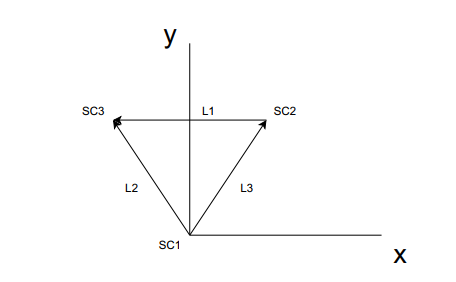
\includegraphics[width=12cm]{TianQin_config.png}
\caption{天琴探测器构型,参考文献\cite{zhang2020full}}
\label{fig2-LISA_con}
\end{center}
\end{figure}

%描述坐标系转换关系,得到臂长表达式或臂长变化量表达式。
由前人的工作\cite{hu2018fundamentals,ye2019optimizing}\cite{luo2016tianqin}\cite{tan2020impact}\cite{zhang2020full},%假如某一波源在黄道坐标系$h(\bar{\theta},\bar{\phi},\hat{\Omega})$可以得到天琴探测器在黄道坐标系(笛卡尔坐标表示)中的表示为:
天琴探测器轨道在探测器质心坐标系下表示如下所示。
\begin{equation}
x(t)=R\cos(\alpha)+\frac{1}{2} R \cdot \emph{e} \cdot \cos(2\alpha-3) +d(\cos(\theta) \cos(\phi)\cos(\gamma)-\sin(\phi)\sin(\gamma)) 
\end{equation}
\begin{equation}
\mathcal(y)(t)= R \sin (\alpha)+\frac{1}{2}R\cdot \emph{e} \cdot \sin (2\alpha)+d(\cos \theta \sin \phi \cos \gamma + \cos \phi \sin  \gamma)
\end{equation}
\begin{equation}
z(t)=-d \sin \theta \cos \gamma
\end{equation}
其中 $\alpha = 2\pi f_{\emph{e}} t+\mathcal{k}$是地球绕太阳的近日点角,$\mathcal{\Omega}$是初始角。
$\emph{e}$是地球离心率,并对其进行小量展开,保留到一阶。
$R$是地球轨道半长轴。
$d$是天琴探测器与地球之间的距离,目前设计为$10^8$米。

%需要说明坐标系转换关系: 从黄道坐标$(\bar{\theta},\bar{\phi})$,如何转换到探测器坐标下臂长的变化量。
在此基础上,探测器的臂长就能由其三角型的构型及其轨道来进行表示。参考时间记$t=0$
则臂长向量可表示为:
\begin{equation}
l_2^a=\cos{\frac{\gamma}{2}}x^a -\sin{\frac{\gamma}{2}y^a}
\end{equation}
\begin{equation}
l_3^a=\cos{\frac{\gamma}{2}}x^a +\sin{\frac{\gamma}{2}y^a}
\end{equation}
其中$\gamma=\frac{\pi}{3}$是SC1的顶角。



%说明迈克尔逊干涉原理
前面已知天琴可构造一对双臂长探测器,因此天琴能够同时探测引力波的两个偏振。基于文献\cite{cornish2001space}\cite{cornish2003lisa}\cite{cutler1998angular},引力波经过探测器会引起臂长变化。考虑波源是在黄道坐标$(\bar{\theta},\bar{\phi})$下,考虑引力波传播方向$\Omega$的自由度,引入极化角来组成新的正交坐标系$\left(
\hat{p},\hat{q},\hat{\psi} \right)$。
\begin{equation}
\hat{p}=\cos \psi\hat{\theta} +\sin{\psi}\hat{\phi}
\end{equation}
\begin{equation}
\hat{q}=-\sin\psi \hat{\theta} + \cos \psi \hat{\phi}
\end{equation}

%在x-y平面内,当$|\bf{x}-\bf{y}|$表示向量$\textbf{x}$和向量$\textbf{y}$笛卡尔距离,则构造单位向量:
%\begin{equation}
%\hat{r}_{ij}(t_i)=\frac{\textbf{x}_j(t_j)-\textbf{x}_i(t_i)}{L_{ij}(t_j)}
%\end{equation}
在静态近似(static limit)和低频近似(low frequency limit)的条件下
单个探测器响应函数可以表示为:

\begin{equation}
\begin{aligned}
h_I(t) &= \frac{\left [\delta L_1(t)-\delta L_2(t) \right ]} {L} \\ 
& =\frac{\sqrt{3}}{2}(\frac{1}{2}h_{xx}-\frac{1}{2}h_{yy}) \\
& =\frac{\sqrt{3}}{2}(A_{+}F^+_I(\theta_S,\phi_S,\psi_S)+A_{\times}F_I^{\times}(\theta_S,\phi_S,\psi_S))
\end{aligned}
\end{equation}

%说明低频近似的表达式
\begin{equation}
F^+_I(\theta_S,\phi_S,\psi_S)=\frac{1}{2}(1+\cos^2\theta_S)\cos 2\phi_S \cos 2\psi_S -\cos\theta_S \sin2\phi_S \sin 2\psi_S
\end{equation}
\begin{equation}
F_I^{\times}(\theta_S,\phi_S,\psi_S)\frac{1}{2}(1+\cos^2\theta_S)\cos 2\phi_S \sin 2\psi_S +\cos\theta_S \sin2\phi_S \cos 2\psi_S
\end{equation}

同理得到探测器"II"的响应后信号为
\begin{equation}
\begin{aligned}
h_{II} &= \frac{\sqrt{3}}{2} \frac{\left [\delta L_1(t) + \delta L_2(t) - 2 \delta L_3(t) \right]} {L}\\ 
& =\frac{\sqrt{3}}{2}(\frac{1}{2}h_{xy} +\frac{1}{2}h_{yx})
\end{aligned}
\end{equation}
且对探测器$II$的响应函数为:
\begin{equation}
F^+_{II}(\theta_S,\phi_S,\psi_S)=F_I^+(\theta_S,\phi_S-\frac{\pi}{4},\psi_S)
\end{equation}
\begin{equation}
F^{\times}_{II}(\theta_S,\phi_S,\psi_S)=F_{II}^{\times}(\theta_S,\phi_S-\frac{\pi}{4},\psi_S)
\end{equation}

由于引力波波长远远大于LISA探测臂长,故而每一组得到的迈克尔逊信号也可表示n阶谐波之和,故而可表示为$h_{\alpha}(t)\ =\ \sum_n \ h_{\alpha,n}(t) \ (\alpha=I,II),$。而其中$h_{\alpha,n}(t)$定义如(\ref{halpha})所示。故而这得到信号函数是($\theta ,\phi ,\varphi$)的函数,而这是三个自变量又随时间演化。对于不同空间探测器,主要体现在这三个角度的函数关系式不同,但是与引力波响应函数表达式是相同的。
%说明全天平均响应函数
%说明TDI*



\begin{comment}
由三角形几何关系可得
\begin{equation}
l\ =\ \frac{L_1 L_2 L_3}{\sqrt{2L_1^2 L_2^2 + 2L_2^2 L_3^2 + 2L_3^2 L_1^2 - L_1^4 -L_2^4 - L_3^4}}
\end{equation}


在激光干涉仪数据流中,数据是测量探测器两臂的激光在同一时间t内的相位差来构造,从而得到了三个航天器相关的TDI观测值。激光沿臂长$L_i$移动所需的时间$\tau_i = L_i/c$,其中$c$是光速。
由于航天器臂长是不相等的。则对应航天器1相关联的TDI响应信号是,
\begin{equation}
X(t)\ =\ s_1(t)\ -\  s_1(t-2\tau_2)\ -\ s_2(t)\ +\ s_2(t-2\tau_1) \label{eq2-tdi-1}
\end{equation}

其中$s_i(t)$是某个时刻到达航天器i的输入信号。则采用$1->2->3->1$顺序表示,其他相应两个航天器的响应信号如公式\ref{eq2-tdi-2}和\ref{eq2-tdi-3}所示。
\begin{equation}
Y(t)\ =\ s_2(t)\ -\  s_2(t-2\tau_3)\ -\ s_3(t)\ +\ s_3(t-2\tau_2) \label{eq2-tdi-2}
\end{equation}
\begin{equation}
Z(t)\ =\ s_3(t)\ -\  s_3(t-2\tau_1)\ -\ s_1(t)\ +\ s_1(t-2\tau_3)  \label{eq2-tdi-3}
\end{equation}

故而由方程(\ref{eq2-tdi-1}-\ref{eq2-tdi-3})可构造三个通道,即A、E、T 通道,到达扣除激光相位噪声的目标,且使得数据之间独立。各个通道表示如公式(\ref{eq2-A} - \ref{eg2-T})所示。
\begin{align}
A\ =\ \frac{1}{3}(2X\ -\ Y\ -\ Z)  \label{eq2-A} \\
E\ =\ -\frac{1}{\sqrt{3}}(Z\ -\ Y) \label{eq2-E} \\
T\ =\ -\frac{\sqrt{2}}{3}(X\ -\ Y\ -\ Z) \label{eq2-T}
\end{align}

A、E 和T通道数据是不相关的。且T通道在低频频段对引力波信号不敏感,只有A和E通道包含引力波信,可用于信号的搜索和分析。


实际上,采用TDI方法计算引力波相位变化对内存和计算力需求很高,故而目前空间探测器都是采用低频近似方法(Low frequency approximation)得到一对双臂探测器输出探测器信号(orthogonal signals)。令$l_1^i$,$l_2^i$,$l_3^i$作为沿着探测臂方向的单位矢量。取$L_i(t)$ 代表探测器第i个臂长。不同臂长可以组成不同探测器。三个臂长可组成两组迈克尔逊信号,且这两组信号相互垂直。如臂长1 和臂长2 可组成一组探测器I。 以LISA响应为例\cite{Cutler1998},则第一组探测器信号(即引力波强度)可以表示为:
\begin{equation}
h_I(t)\ =\ [\delta L_1(t)-\delta L_2(t)]/L = \frac{1}{2}h_{ij}(t)(l_1^il_1^j - l_2^il_2^j)=\frac{\sqrt{3}}{2}(\frac{1}{2}h_{xx}-\frac{1}{2}h_{xy}) \label{hI}
\end{equation}
第二组探测器信号则可表示为:
\begin{align}
  h_{II}(t) &=\  3^{-1/2}[\delta L_1(t) +\delta L_2(t) - 2\delta L_3(t)]/L        \\
             &=\  \frac{1}{2\sqrt{3}} h_{ij}(t)(l_1^il_1^j + l_2^il_2^j - 2l_3^il_3^j) =\frac{\sqrt{3}}{2}(\frac{1}{2}h_{xy}+\frac{1}{2}h_{yx}) \label{hII}
\end{align}
公式($\ref{hI}$)和($\ref{hII}$)中需要运用的坐标转换关系,其中$l_i^{\alpha}=cos\gamma_i x^a+sin\gamma_i y^a$,$\gamma_i=\pi/12+ (i-1)\pi/3$,$l_i^a$是沿探测臂的单位矢量,$x^a$和$y^a$分别是探测器坐标系下沿着x轴和y轴的单位矢量,$a=x,y,z$是三维空间指标。

由上一章可知,探测器响应函数跟引力波信号是线性关系,并且考虑空间探测器方位角$(\theta , \phi)$和偏振角$\varphi$,则响应后的引力波信号可表示为
\begin{equation}
h_{\alpha,n}(t)=\frac{1}{D}\frac{\sqrt{3}}{2} [ F^+_{\alpha}(t)A_n^{+}(t) + F^{\times}_{\alpha}(t)A_n^{\times}(t)] \label{halpha}
\end{equation}
%其中$A_n^{+,\times}$是由对EMRI 源进行特征表示的波形模型中的两种偏振模式系数。而系数$\frac{\sqrt{3}}{2}$是LISA臂长实际倾角是60°而不是90°。$F_{\alpha}^{+,\times}$是LISA探测器响应函数,具体表示如公式所示。
\begin{align}
 F_I{+}\      &=\  \frac{1}{2}(1+cos^2\theta)cos(2\phi)cos(2\varphi)-cos\theta sin(2\phi)sin(2\varphi)       \\
 F_I{\times}\ &=\  \frac{1}{2}(1+cos^2\theta)cos(2\phi)sin(2\varphi)+cos\theta sin(2\phi) cos(2\varphi)       \\
  F_{II}{+}\      &=\  \frac{1}{2}(1+cos^2\theta)sin(2\phi)cos(2\varphi)+cos\theta cos(2\phi)sin(2\varphi)       \\
 F_{II}{\times}\ &=\  \frac{1}{2}(1+cos^2\theta)sin(2\phi)sin(2\varphi)-cos\theta cos(2\phi) cos(2\varphi)
\end{align}


由于引力波波长远远大于LISA探测臂长,故而每一组得到的迈克尔逊信号也可表示n阶谐波之和,故而可表示为$h_{\alpha}(t)\ =\ \sum_n \ h_{\alpha,n}(t) \ (\alpha=I,II),$。而其中$h_{\alpha,n}(t)$定义如(\ref{halpha})所示。故而这得到信号函数是($\theta ,\phi ,\varphi$)的函数,而这是三个自变量又随时间演化。对于不同空间探测器,主要体现在这三个角度的函数关系式不同,但是与引力波响应函数表达式是相同的。

在考虑不旋转的探测器坐标系下,基于初始空间方位角$(\theta_S,\phi_S)$和初始相位角$\phi_0$,上述三个角度的演化公式如\ref{theta-t}所示。
\begin{equation}
cos \theta(t) = \frac{1}{2}cos \theta_S -\frac{\sqrt{3}}{2} sin \theta_S cos[\bar{\phi_0} + 2\pi(t/T) - \phi_S]
\label{theta-t}
\end{equation}
\begin{equation}
\phi(t) = \bar{a_0} + 2\pi(t/T) + tan^{-1}[\frac{\sqrt{3}cos \theta_S + sin \theta_S cos[\bar{\phi_0} + 2 \pi(t/T) - \phi_S]}{2 sin \theta_S sin[\bar{\phi_0}+ 2\pi(t/T)-\phi_S]}
\end{equation}
\begin{equation}
tan \psi =\frac{A} {B}
\end{equation}
其中
\begin{equation}
A= \{ \frac{1}{2} cos \theta_L - \frac{\sqrt{3}}{2} sin \theta_L cos[\bar{\phi_0} + 2\pi (t/T)-\phi_L] - cos \theta(t) [cos \theta_L cos \theta_S + sin \theta_L sin \theta_S cos(\phi_L - \phi_S]  \}
\end{equation}



\begin{equation}
\begin{split}
B=&[\frac{1}{2}sin \theta_L sin \theta_S sin(\phi_L - \phi_S) - \frac{\sqrt{3}}{2}cos(\bar{\phi_0} + 2\pi (t/T)) (cos \theta_L sin \theta_S sin \phi_S - cos \theta_S sin \theta_L sin \phi_L ) \\
&- \frac{\sqrt{3}}{2}sin (\bar{\phi_0} + 2 \pi (t/T)) (cos \theta_S sin \theta_L cos \phi_L - cos \theta_L sin \theta_S cos \phi_S)]
\end{split}
\end{equation}


%\begin{figure}[htbp]
%\begin{center}
%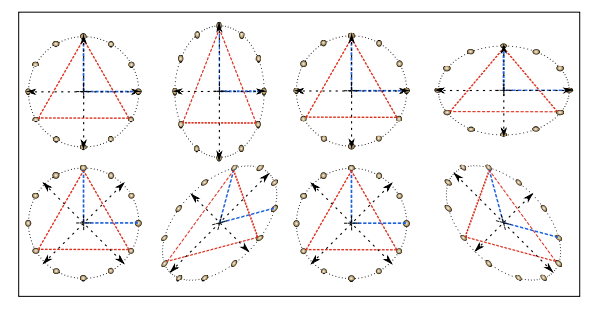
\includegraphics[width=12cm]{Figures/Chapter02/LISA.PNG}
%\caption{引力波经过LISA探测器平面引起的变化;图片来自\cite{Mitryk2012}}
%\label{fig1.1}
%\end{center}
%\end{figure}

\end{comment}



%\section{天琴对EMRI的探测能力}
范会敏等人\cite{Fan:2020zhy}基于理想信噪比的计算和FIM(Fisher Information Matrix)的方法评估了天琴对EMRI这类波源的探测事件率和物理参数估计精度。%
%事件率计算和结果。
%参数估计计算和结果
